\section*{Aufgabe 2}

\subsection*{a)}
Um die durchschnittliche Precision zu berechnen muss man erst die Precision pro Anfrage berechnen.
Diese berechnet sich: R/D wobei R die Anzahl an bisher gefundener relevanter Documente ist und D die Anzahl aller bisher gefundenen Documente. Damit ergibt sich folgende Tabelle. ( P1: Percision für Anfrage 1, P2 für Anfrage 2)

\begin{tabular}{|c|c|c|c|c|c|c|c|c|c|c|}
\hline Rang 	& 1 & 2  & 3  & 4  & 5  & 6  & 7  & 8  & 9  & 10 \\ 
\hline Anfrage1 & 1 & 1  & 0  & 1  & 0  & 1  & 0  & 0  & 0  & 1  \\ 
\hline Anfrage2 & 0 & 1  & 0  & 1  & 1  & 0  & 1  & 0  & 0  & 0 \\ 
\hline P1	    & 1 & 1	 & 0,67 & 0,75 & 0,6& 0,67&	0,57 & 0,5& 0,44 & 0,5\\
\hline P2		& 0	& 0,5 & 0,33 & 0,5 & 0,6 & 0,5 & 0,57 & 0,57 & 0,44 & 0,44 \\
\hline 
\end{tabular} 
\\

Die durchschnittliche Precision AP berechnet sich als Arichmetisches Mittel von P1 und P2. 
\\

\begin{tabular}{|c|c|c|c|c|c|c|c|c|c|c|c|}
\hline Recall 	  & 0    & 0,1  &  0,2 & 0,3 & 0,4 & 0,5 & 0,6 & 0,7  & 0,8  & 0,9  & 1 \\
\hline AP ISR3000 & 0,5 & 0,75 & 0,5 & 0,63 & 0,6 & 0,58 & 0,57 & 0,54 & 0,44 & 0,47\\
\hline

\end{tabular}

\subsection*{b)}
\begin{tabular}{|c|c|c|c|c|c|c|c|c|c|c|c|}
\hline Recall 	  & 0    & 0,1  &  0,2 & 0,3 & 0,4 & 0,5 & 0,6 & 0,7  & 0,8  & 0,9  & 1 \\
\hline AP ISR2000 & 0,75 & 0,75 & 0,75 & 0,7 & 0,7 & 0,7 &0,7 & 0,65 & 0,65 & 0,65 & 0,65\\

\hline

\end{tabular}

\begin{figure}[H]
\centering
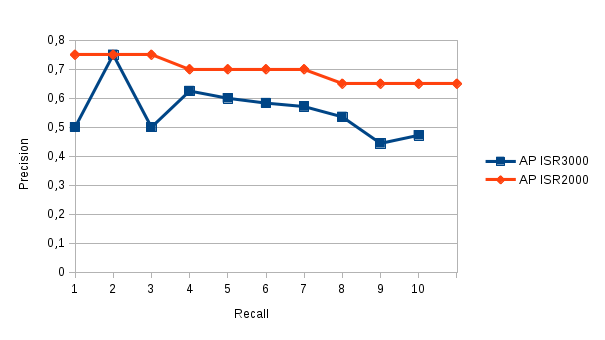
\includegraphics[width=0.7\linewidth]{./Aufgabe2/ir3vsir2}
\caption{ISR3000 vs ISR2000}
\label{fig:ir3vsir2}
\end{figure}

Der vergleich der beiden IR Systeme zeigt, dass ISR2000 eine höhere durchschnittliche Precision als ISR3000 hat. (vgl.:Abbildung \ref{fig:ir3vsir2})
Somit ist ISR2000 besser.

\subsection*{c)}
Fügt man eine weitere Anfrage hinzu, wird für diese ebenfalls die Precision berechnet und der AP-Wert neu ermittel als Arithmetisches mittel von (P1+P2+P3) / 3.

\begin{tabular}{|c|c|c|c|c|c|c|c|c|c|c|}
\hline Rang 	& 1 & 2  & 3  & 4  & 5  & 6  & 7  & 8  & 9  & 10 \\ 
\hline Anfrage3 & 1 & 1  & 0  & 1  & 0  & 1  & 0  & 0  & 0  & 1  \\ 
\hline P3 & 0 & 1  & 0  & 1  & 1  & 0  & 1  & 0  & 0  & 0 \\ 
\hline
\end{tabular}
\\
Das ergibt:
\\
\begin{tabular}{|c|c|c|c|c|c|c|c|c|c|c|c|}
\hline Recall 	  & 0    & 0,1  &  0,2 & 0,3 & 0,4 & 0,5 & 0,6 & 0,7  & 0,8  & 0,9  & 1 \\
\hline AP ISR3000 v2 & 0,33 & 0,67 & 0,56 & 0,58 & 0,6 & 0,56 & 0,57 & 0,57 & 0,48 & 0,48\\
\hline

\end{tabular}
\newpage